
\section{Subcritical flow without a shock over a bump}

This is a subcritical flow over a bump. This test is adapted from Goutal and Maurel~\cite{GM1997}. No shock occurs in this scenario. 

Consider a one dimensional domain $[0,25]$ with topography
\begin{equation}
z(x)= \left\{ \begin{array}{ll}
 0.2-0.05\left(x-10\right)^2& ~\textrm{if}\quad 8 \leq x \leq 12\,,\\
 0 & ~\textrm{otherwise}\,,\\
\end{array} \right.
\end{equation}
together with Dirichlet boundary conditions.
Physically, the boundary conditions mean that there is a source of flow upstream at the point $x=0^{-}$ and at the same time there exists a sink of flow downstream at the point $x=25^{+}$\,.


The analytical height is found by solving the Bernoulli equation. The simplified Bernoulli equation is the following cubic equation
\begin{equation}
h^3 + \left(z - \frac{q^2}{2 g H^2} - H \right) h^2 + \frac{q^2}{2 g} = 0\,,
\end{equation}
where $H$ is the upstream height and $q=uh$ is the discharge or $x$-momentum. When the height $h$ has been found, the velocity is computed as $u=q/h$\,.

\subsection{Results}
For our test we consider the initial condition
\begin{equation}
u(x,y,0)=v(x,y,0)=0\,, \quad
w(x,y,0)= 0.2\,,
\end{equation}
and the Dirichlet boundary conditions at $x=0^{-}$ and $25^{+}$ to be 
\begin{equation}
[w,hu,hv]=[2, 4.42, 0]\,.
\end{equation}
Representatives of the simulation results are given in the following three figures. Even though we have small discrepancy in the numerical and analytical momenta, these numerical an analytical solutions should agree quite well.

\begin{figure}
\begin{center}
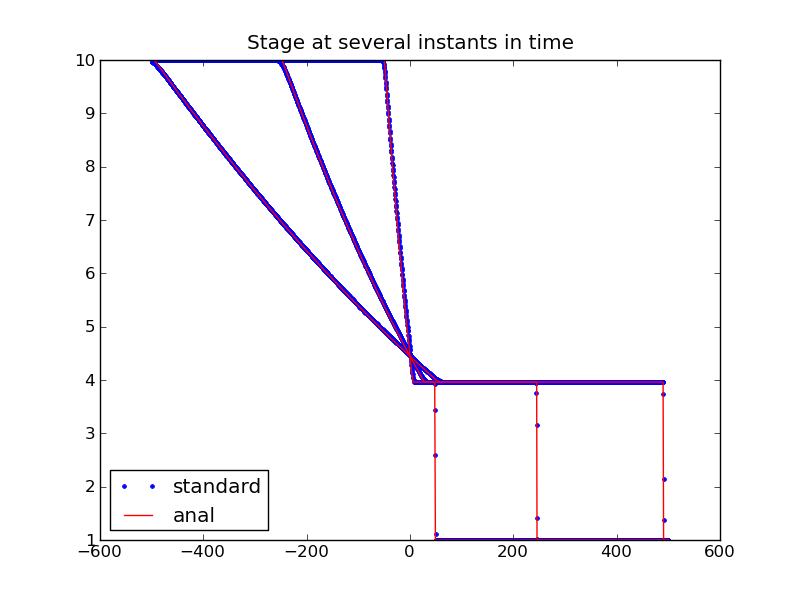
\includegraphics[width=0.9\textwidth]{stage_plot.png}
\end{center}
\caption{Stage results}
\end{figure}


\begin{figure}
\begin{center}
\includegraphics[width=0.9\textwidth]{xmom_plot.png}
\end{center}
\caption{Xmomentum results}
\end{figure}


\begin{figure}
\begin{center}
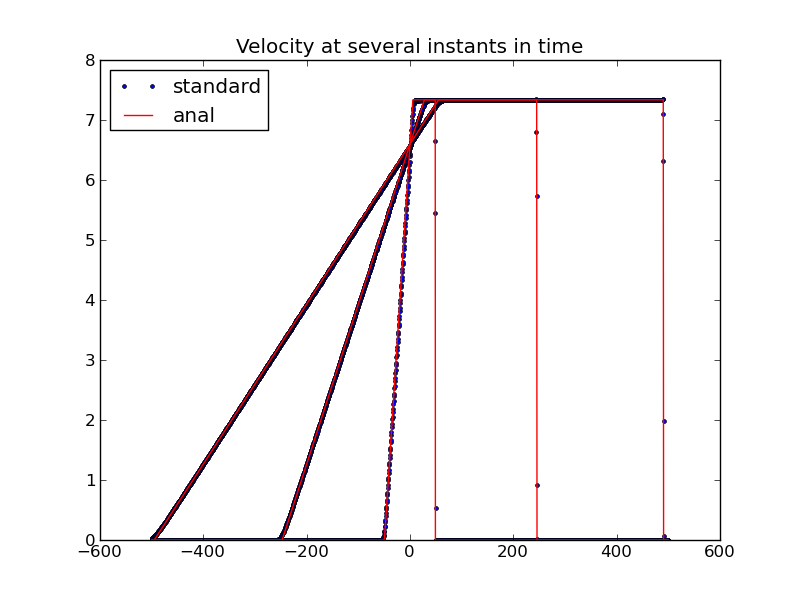
\includegraphics[width=0.9\textwidth]{xvel_plot.png}
\end{center}
\caption{Xvelocity results}
\end{figure}


\endinput
